\chapter{Plataforma de trabajo} \label{chap:plataforma_trabajo}
% Describir las herramientas y el entorno de trabajo


\section{El videojuego: Tales of Tribute} \label{sec:tales_of_tribute}
% Explicar las reglas básicas del juego, sus mecánicas principales (mazos, agentes, prestigio, poder...)


\section{El entorno de simulación: Scripts of Tribute} \label{sec:scripts_of_tribute}
% Motor Scripts of Tribute como plataforma
% Proyecto de código abierto que permite enfrentar bots entre sí


\subsection{La competición IEEE-CoG} \label{sec:competicion_ieee_cog}
% Plataforma ya usada en competiciones académicas
% Resultados de otros años

\begin{figure}
	\centering
	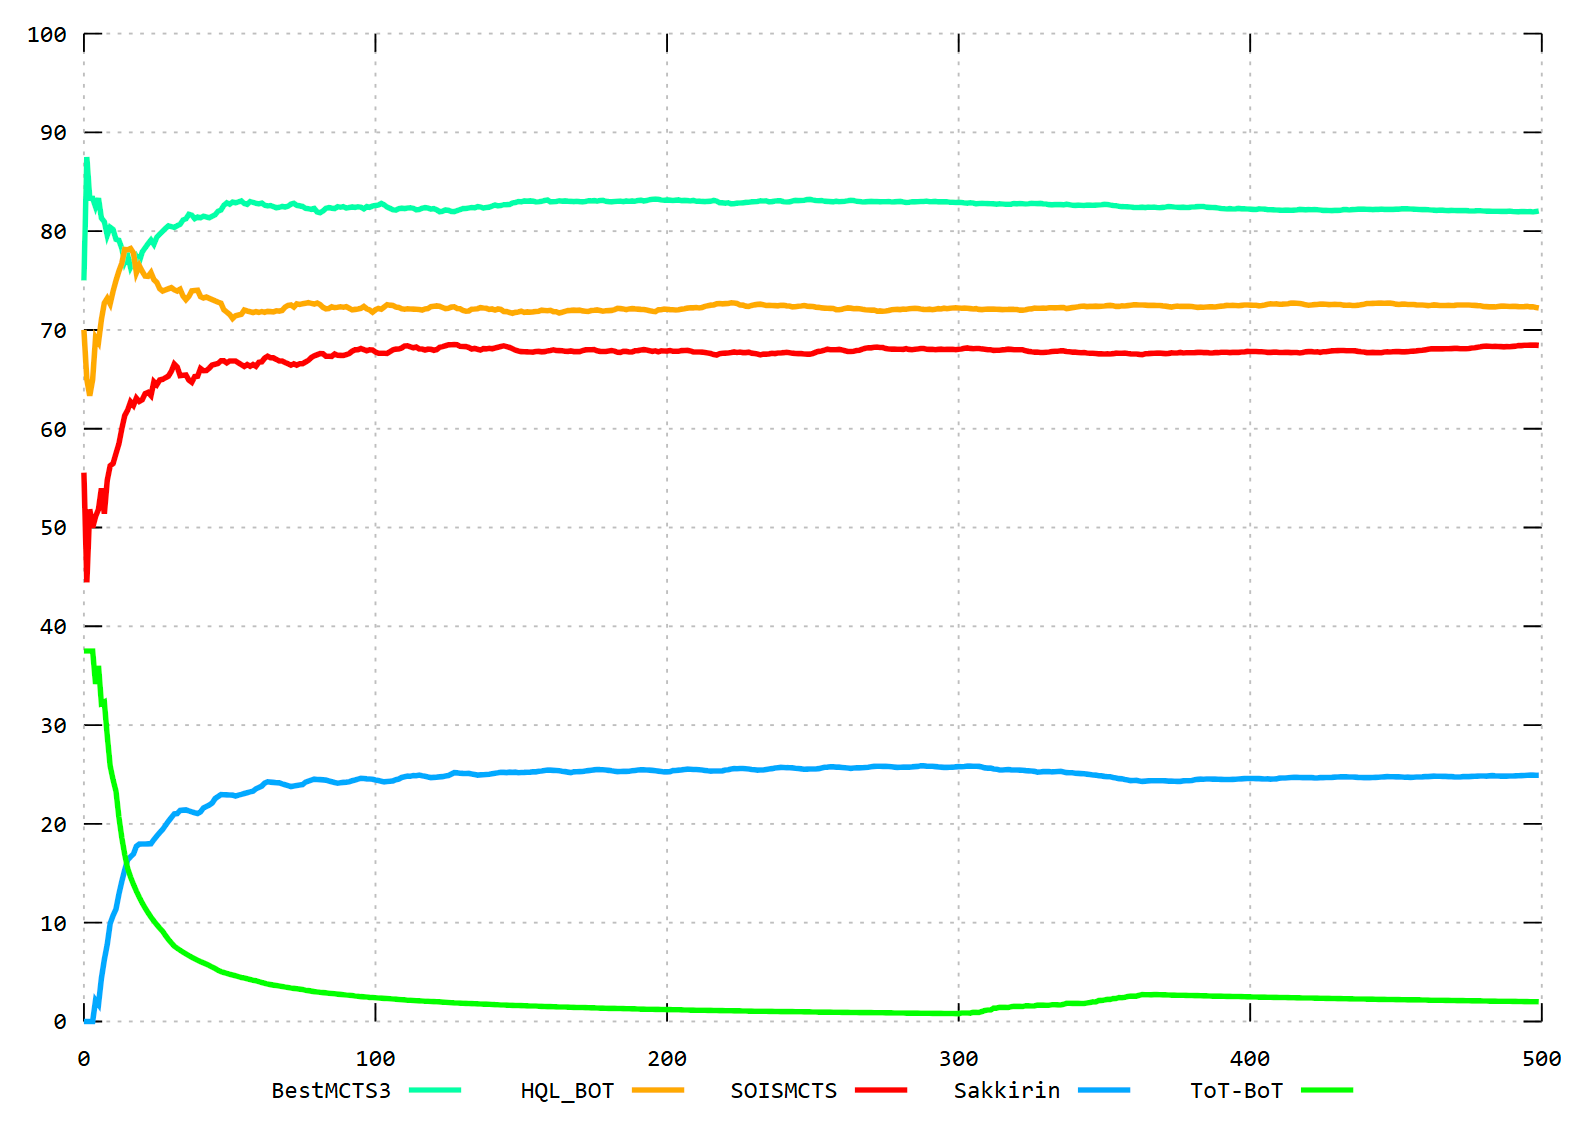
\includegraphics[width=0.8\textwidth]{img/ieee-cog-2024.png}
	\caption{Resultados de la competición IEEE-CoG 2024.}
	\label{fig:competicion_ieee_cog_2024}
\end{figure}

\subsection{Arquitectura del entorno} \label{sec:arquitectura_entorno}
% Explicar cómo funciona la comunicación entre el motor y los bots